
\documentclass[12pt,journal,compsoc]{IEEEtran}
\usepackage{array}
\usepackage{bytefield}
\usepackage{graphicx}
\usepackage{listings}
\usepackage{slashbox}
\usepackage{tikz}
\lstset{
frame=tb,
language=C,
aboveskip=3mm,
belowskip=3mm,
showstringspaces=false,
columns=flexible,
basicstyle={\small\ttfamily},
numbers=none,
breaklines=true,
breakatwhitespace=true,
tabsize=3
}
\hyphenation{op-tical net-works semi-conduc-tor}
\newcounter{mcount}
\setcounter{mcount}{0}
\begin{document}
\title{Chat System}
\author{David Gong, Stephen Hamilton}% <-this % stops a space
\date{Sunday, September 21, 2014}
\IEEEtitleabstractindextext{%
\begin{abstract}
Our goal is to develop a distributed chat server client system that is fault tolerant. 
\end{abstract}
}
\maketitle
\section{Introduction}
\IEEEPARstart{T}{his} system will be composed of a client and a server.  Servers will communicate through spread and utilize multicast with agreed ordering.  There will be 5 servers that will communicate with each other and maintain a total order for all chat rooms.  Clients can connect to any of the five servers, login, and create chat rooms, like already seen messages, change names, and leave chat rooms.  The system will be fault tolerant in that each server can go down, and the system will continue to work as long as 3 or more servers are running.  A server can leave the network and come back, and as long as a majority is present, the service will continue to work.
\section{Design}
\subsection{Assumptions}
Below are our assumptions.
\begin{itemize}
\item A chat client can go offline or crash, but will not produce malicious code and/or messaging that can cause the spread daemon to work incorrectly (i.e. spoof partitioning/join messaging).
\end{itemize}
\subsection{Chat Message Packet}
\begin{lstlisting}
// Structure of chat packet.
int type;//Type of packet 0 for message, 1 for like
int sequence;//Global ordering of message
char name[25]; //Text name of user
char group[25]; //Text name of chat room
char text[80]; //Text of chat message
int like_sequence; //Integer of sequence number of message liked
\end{lstlisting}
The message packet is utilized for both chat messages and "like" messages created by a user.  The message packet will be saved to disk when received from spread, and the sequence number will be assigned upon receiving it from spread (it is null initially).

\subsection{Server State Machine}
\begin{center}
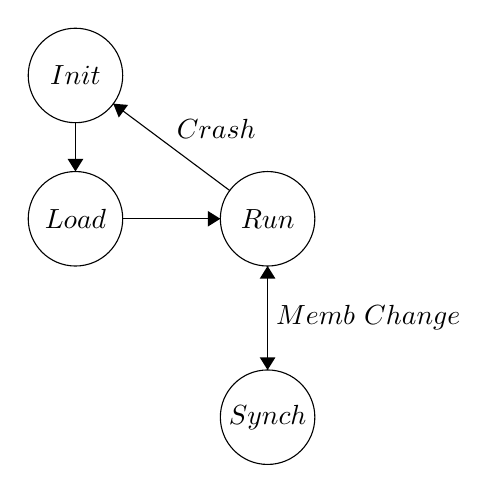
\begin{tikzpicture}[scale=0.2]
\tikzstyle{every node}+=[inner sep=0pt]
\draw [black] (3.3,-3.2) circle (3);
\draw (3.3,-3.2) node {$Init$};
\draw [black] (3.3,-12.3) circle (3);
\draw (3.3,-12.3) node {$Load$};
\draw [black] (15.5,-12.3) circle (3);
\draw (15.5,-12.3) node {$Run$};
\draw [black] (15.5,-24.9) circle (3);
\draw (15.5,-24.9) node {$Synch$};
\draw [black] (3.3,-6.2) -- (3.3,-9.3);
\fill [black] (3.3,-9.3) -- (3.8,-8.5) -- (2.8,-8.5);
\draw [black] (6.3,-12.3) -- (12.5,-12.3);
\fill [black] (12.5,-12.3) -- (11.7,-11.8) -- (11.7,-12.8);
\draw [black] (15.5,-15.3) -- (15.5,-21.9);
\fill [black] (15.5,-21.9) -- (16,-21.1) -- (15,-21.1);
\draw (16,-18.6) node [right] {$Memb\mbox{ }Change$};
\draw [black] (15.5,-21.9) -- (15.5,-15.3);
\fill [black] (15.5,-15.3) -- (15,-16.1) -- (16,-16.1);
\draw [black] (13.1,-10.51) -- (5.7,-4.99);
\fill [black] (5.7,-4.99) -- (6.05,-5.87) -- (6.64,-5.07);
\draw (12.24,-7.25) node [above] {$Crash$};
\end{tikzpicture}
\end{center}

\subsection{Data Structure}
We intend to use a vector that contains each machine id and the number of messages received from each machine.  This will be used at each machine to let other machines know what messages they have received so far.
We also will have an array for all the chat messages that will contain the message packet struct.
\subsection{Design Details}
Each server will maintain the above data structure.  Upon a membership change, servers will 
\\
Upon any membership change, all servers write all messages received to disk at that point.  
\end{document}
